%%%%%%%%%%%%%%%%%%%%%%%%%%%%%%%%%%%%%%%%%
% Beamer Presentation
% LaTeX Template
% Version 1.0 (10/11/12)
%
% This template has been downloaded from:
% http://www.LaTeXTemplates.com
%
% License:
% CC BY-NC-SA 3.0 (http://creativecommons.org/licenses/by-nc-sa/3.0/)
%
%%%%%%%%%%%%%%%%%%%%%%%%%%%%%%%%%%%%%%%%%

%----------------------------------------------------------------------------------------
%   PACKAGES AND THEMES
%----------------------------------------------------------------------------------------

\documentclass{beamer}

\mode<presentation> {

%dencoding
%--------------------------------------
\usepackage[utf8]{inputenc}
\usepackage[T1]{fontenc}
%--------------------------------------

%Portuguese-specific commands
%--------------------------------------
\usepackage[portuguese]{babel}
%--------------------------------------

%Hyphenation rules
%--------------------------------------
\usepackage{hyphenat}
\hyphenation{mate-mática recu-perar}
%--------------------------------------

\bibliographystyle{plain}

% The Beamer class comes with a number of default slide themes
% which change the colors and layouts of slides. Below this is a list
% of all the themes, uncomment each in turn to see what they look like.

%\usetheme{default}
%\usetheme{AnnArbor}
%\usetheme{Antibes}
%\usetheme{Bergen}
%\usetheme{Berkeley}
%\usetheme{Berlin}
%\usetheme{Boadilla}
%\usetheme{CambridgeUS}
%\usetheme{Copenhagen}
%\usetheme{Darmstadt}
%\usetheme{Dresden}
%\usetheme{Frankfurt}
%\usetheme{Goettingen}
%\usetheme{Hannover}
%\usetheme{Ilmenau}
%\usetheme{JuanLesPins}
%\usetheme{Luebeck}
%\usetheme{Madrid}
\usetheme{Malmoe}
%\usetheme{Marburg}
%\usetheme{Montpellier}
%\usetheme{PaloAlto}
%\usetheme{Pittsburgh}
%\usetheme{Rochester}
%\usetheme{Singapore}
%\usetheme{Szeged}
%\usetheme{Warsaw}


% As well as themes, the Beamer class has a number of color themes
% for any slide theme. Uncomment each of these in turn to see how it
% changes the colors of your current slide theme.

%\usecolortheme{albatross}
%\usecolortheme{beaver}
%\usecolortheme{beetle}
%\usecolortheme{crane}
\usecolortheme{dolphin}
%\usecolortheme{dove}
%\usecolortheme{fly}
%\usecolortheme{lily}
%\usecolortheme{orchid}
%\usecolortheme{rose}
%\usecolortheme{seagull}
%\usecolortheme{seahorse}
%\usecolortheme{whale}
%\usecolortheme{wolverine}

%\setbeamertemplate{footline} % To remove the footer line in all slides uncomment this line
\setbeamertemplate{footline} % To replace the footer line in all slides with a simple slide count uncomment this line

\setbeamertemplate{footline}{
\leavevmode%
  \hbox{%
  \begin{beamercolorbox}[wd=.4\paperwidth,ht=2.25ex,dp=1ex,center]{author in head/foot}%
    \usebeamerfont{author in head/foot}\insertshortauthor
  \end{beamercolorbox}%
  \begin{beamercolorbox}[wd=.6\paperwidth,ht=2.25ex,dp=1ex,center]{title in head/foot}%
    \usebeamerfont{title in head/foot}\insertshorttitle\hspace*{6em}
    \insertframenumber{} / \inserttotalframenumber\hspace*{1ex}
  \end{beamercolorbox}}%
  \vskip0pt
}

\setbeamertemplate{navigation symbols}{} % To remove the navigation symbols from the bottom of all slides uncomment this line
}

\usepackage{graphicx} % Allows including images
\usepackage{booktabs} % Allows the use of \toprule, \midrule and \bottomrule in tables

%----------------------------------------------------------------------------------------
%   TITLE PAGE
%----------------------------------------------------------------------------------------

\title[Expressões Regulares]{Expressões Regulares na Prática!} % The short title appears at the bottom of every slide, the full title is only on the title page

\author{Gustavo Yudi Bientinezi Matsuzake} % Your name
\institute[UTFPR] % Your institution as it will appear on the bottom of every slide, may be shorthand to save space
{
Universidade Tecnológica Federal do Paraná\\ % Your institution for the title page
Coders UTFPR\\
\medskip
\textit{matsuzake@alunos.utfpr.edu.br} % Your email address
\url{https://github.com/yudi-matsuzake/coders-regex}
}
\date{\today} % Date, can be changed to a custom date

\begin{document}

\begin{frame}
\titlepage % Print the title page as the first slide
\end{frame}

\newcommand{\sumario}{
\begin{frame}
\frametitle{Sumário} % Table of contents slide, comment this block out to remove it
\tableofcontents % Throughout your presentation, if you choose to use \section{} and \subsection{} commands, these will automatically be printed on this slide as an overview of your presentation
\end{frame}
}

\sumario

%----------------------------------------------------------------------------------------
%   PRESENTATION SLIDES
%----------------------------------------------------------------------------------------

\section{Introdução} 
\frame{\tableofcontents[currentsection]}

\subsection{O que é?} % A subsection can be created just before a set of slides with a common theme to further break down your presentation into chunks

%-----------------------------------------------
\begin{frame}
	\frametitle{Definição}

	\Large{\azul{\textbf{Expressão Regular}} é:}

	\begin{itemize}
		\item Uma "linguagem de programação"\cite{hopcroft};
		\item Intimamente relacionada aos \azul{DFA}, que são \textit{\azul{autômatos}}, analisadores sintáticos\cite{hopcroft};
		\item Uma maneira sucinta e \azul{finita} de representar uma linguagem infinita - regular;
		\item É um método formal de se especificar um padrão de texto\cite{aurelio}.
	\end{itemize}

\end{frame}

%------------------------------------------------
\begin{frame}
	\begin{block}{Mesmo, Eu.}
	"Uma imagem vale mais do que mil palavras. Uma Expressão Regular\footnote{bombeável} vale infinitas."
	\end{block}
\end{frame}
%------------------------------------------------

\begin{frame}
	\frametitle{Observação importante:}
	\centering \Large{Diferença da teoria e da prática.}
\end{frame}

%------------------------------------------------
\subsection{Parte prática!}

\begin{frame}
	\Large{\azul{\textbf{Vamos deixar claro nosso escopo!}}}
\end{frame}

%------------------------------------------------
\begin{frame}
	\frametitle{Para a felicidade de alguns, infelicidade de outros...}
	
	\begin{itemize}
		\item Nosso escopo nessa apresentação é mais \azul{prático} e não teórico;
		\item Vamos aprender \azul{como} usar;
		\item Vamos aprender \azul{onde} usar;
		\item Vamos aprender \azul{porque} usar.
	\end{itemize}
\end{frame}

\subsection{Você não vai aprender isso nessa apresentação!}

%------------------------------------------------
\begin{frame}
\frametitle{Nada de lógica}
\centering
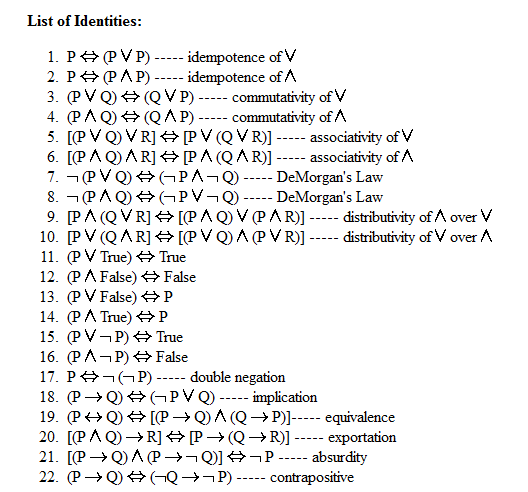
\includegraphics[width=0.8\textwidth]{./imagens/re/logica.png}
\end{frame}
%------------------------------------------------
\begin{frame}
\frametitle{Nada de transição de DFA para NFA}
\centering
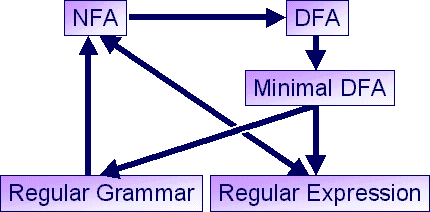
\includegraphics[width=0.8\textwidth]{./imagens/re/NFA-DFA.png}
\end{frame}
%------------------------------------------------
\begin{frame}
\frametitle{Não vamos aprender autômatos}
\centering
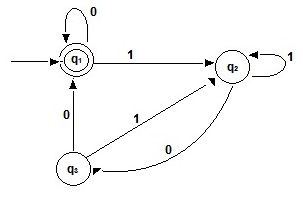
\includegraphics[width=0.8\textwidth]{./imagens/re/NFA.jpg}
\end{frame}
%------------------------------------------------

\subsection{Você vai aprender muito isso!}
%------------------------------------------------
\begin{frame}
\frametitle{Isso vai fazer parte da sua realidade}
\centering
\bf
\Large{\textasciicircum *[A-Za-z0-9\_]+:(.*)\$}
\end{frame}
%------------------------------------------------
\begin{frame}
\frametitle{Isso não vai te dar mais pânico!}
\centering
\bf
\Large{([0-9]\{1,3\}\textbackslash.)\{2\}[0-9]\{1,3\}-[0-9]\{2\}}
\end{frame}
%------------------------------------------------
\begin{frame}
\frametitle{Isso será fácil de entender (:}
\centering
\bf
\Large{[-+]?[0-9]\{1,3\}(\textbackslash.[0-9]\{3\})?(,[0-9]\{2\})?}
\end{frame}
%------------------------------------------------
\begin{frame}
\begin{figure}
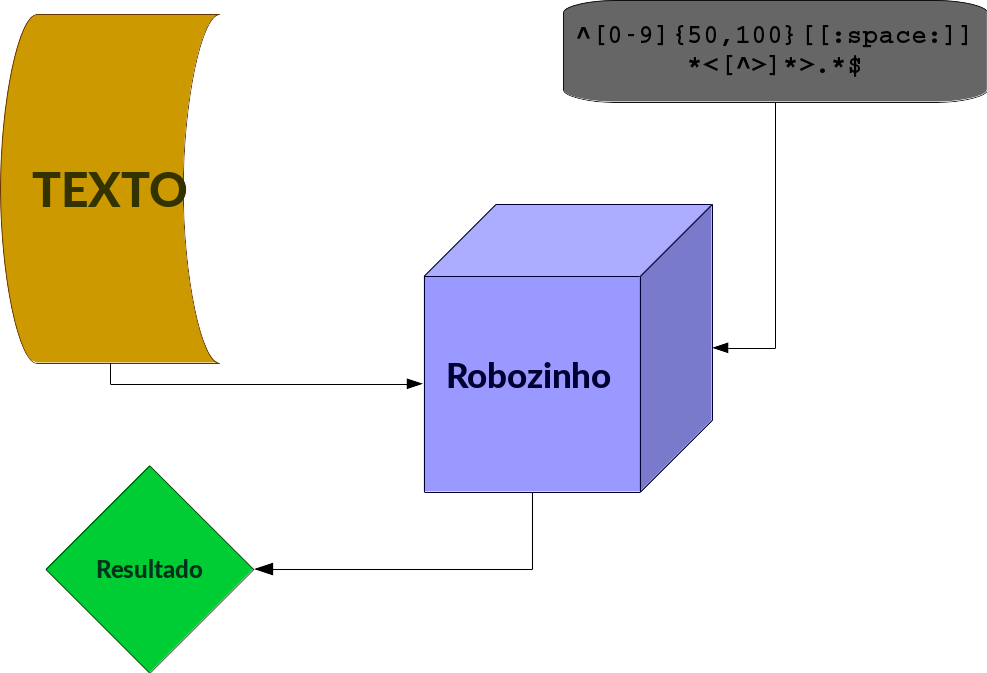
\includegraphics[height=0.75\textheight]{./imagens/re/como-vai-funcionar.png}
\caption{Como vamos abordar as RE}
\end{figure}
\end{frame}

\subsection{Livro}

\begin{frame}
\frametitle{[Expressões Regulares] Uma abordagem divertida}

\begin{figure}[h]
\centering

\includegraphics[height=0.75\textheight]{./imagens/re/piazinho.jpg}
\caption{Essa apresentação foi \azul{inspirada}, \azul{causada} e \azul{é} sobre esse livro.}
\end{figure}
\end{frame}



%------------------------------------------------

\section{Referências}

\begin{frame}
\frametitle{Referências}
\bibliography{regex-coders}
\end{frame}

%------------------------------------------------

\section{FIM}
\begin{frame}
\frametitle{Acabou :(}
\centerline{Dúvidas?}

\titlepage
\end{frame}

%----------------------------------------------------------------------------------------

\end{document}
